\section{Auswertung}
\label{sec:Auswertung}
\subsection{Bestimmung des vertikalen Magnetfeldes}
Zunächst muss mittels der Gleichung
\begin{equation*}
    B = \mu_0 \frac{8N}{\sqrt{125}R}I
\end{equation*} 
die Feldstärke des vertikalen Magnetfeldes der Erde mittels des gemessenen Spulenstroms $I$ berechnet werden. \cite{leifi}
Dabei sind $N$ die Anzahl an Windungen, $R$ der Radius der Spule und $\mu_0$ die magnetische Feldkonstante.
Die Vertikalfeld-Spule hat einen Radius von $R = \qty{11.735}{\centi\metre}$ und eine Windungszahl von $N = 20$.\cite{sample}
Somit lässt sich eine Feldstärke von 
\begin{equation*}
    B_{\text{vertikal}} = \qty{34.79}{\micro\tesla}
\end{equation*}
berechnen.
\subsection{Bestimmung der Lande Faktoren}
In Tabelle \ref{tab:hphase} sind die gemessenen Feldstärken der horizontalen Felder bei den gegeben Frequenzen aufgezeigt.
\begin{table}
        \centering
        \caption{Gemessene horizontale Feldstärken der festen und der Sweep-Spule in Abhängigkeit von der Frequenz.}
        \label{tab:hphase}
        \begin{tabular}{S[table-format=4.0] S[table-format=2.2] S[table-format=1.2] S[table-format=2.2] S[table-format=2.2]}
        \toprule
        & \multicolumn{2}{c}{$^{87}\text{Rb}$} & \multicolumn{2}{c}{$^{85}\text{Rb}$} \\
        \cmidrule(lr){2-3}\cmidrule(lr){4-5}
        {$f \mathbin{/} \si{\kilo\hertz}$} & {$I_\text{hori} \mathbin{/} \si{\ampere}  $} & {$I_\text{sweep} \mathbin{/} \qty{0.1}{\ampere}$}
        & {$I_{\text{hori}} \mathbin{/} \si{\ampere}$} & {$I_{\text{sweep}} \mathbin{/} \qty{0.1}{\ampere}$} \\
        \midrule
            100    &     0         &  6.47     &       0        &   7.78    \\
            200    &     -0.01     &  6.77     &       -0.01    &   9.14    \\
            300    &     -0.04     &  4.6      &       -0.04    &   8.13    \\
            400    &     -0.06     &  3.27     &       -0.06    &   9       \\
            500    &     -0.08     &  3.45     &       -0.08    &   9.37    \\
            600    &     -0.1      &  3.0      &       -0.1     &   10      \\
            700    &     -0.13     &  2.5      &       -0.13    &   10.35   \\
            800    &     -0.14     &  2.4      &       -0.2     &   3.55    \\
            900    &     -0.15     &  2.7      &       -0.23    &   1.86    \\
            1000   &     -0.15     &  5.1      &       -0.26    &   1.90    \\                                                                                
        \bottomrule
        \end{tabular}
\end{table}
\begin{figure}
    \centering
    \caption{Gemessene und gefittete Feldstärken für beide Isotope.}
    \label{fig:fit}
    \includegraphics[width = 0.8 \textwidth]{build/fits.pdf}
\end{figure}
Um die Lande Faktoren der beiden Isotope zu bestimmen, wird die Gleichung \eqref{eqn:magnetf} gefittet.
Die Ausgleichsgerade besitzt die Form
\begin{equation*}
    B =  af + b \; ,
\end{equation*} 
wobei $a$ und $b$ die Fitparameter sind.
Diese ergeben sich zu 
\begin{align*}
    a_{85} &= \qty{2.16(3)e-10}{\tesla\second}   \\
    b_{85} &= \qty{2.13(20)e-5}{\tesla}            \\
    a_{87} &= \qty{1.42(4)e-10}{\tesla\second}   \\
    b_{87} &= \qty{2.12(27)e-5}{\tesla}            \; .
\end{align*}
Nun steckt in dem Parameter $a$ der Landefaktor, welche die Beziehung 
\begin{equation*}
    a = \frac{h}{\mu_\text{B}g_F} \iff g_F = \frac{h}{\mu_\text{B}a}
\end{equation*}
haben.
Somit können die Lande Faktoren zu 
\begin{align}
    g_{F, 85} &= \num{0.330(5)} \\ 
    g_{F, 87} &= \num{0.501(15)}    \label{eqn:gf87}
\end{align}
bestimmt werden.
\subsection{Bestimmung der Kernspins}
Im Folgenden wird der Kernspin beider Isotope mit der Gleichung 
\begin{equation}
    \frac{1}{2}\left ( \frac{g_J}{g_F} - 1 \right ) \label{eqn:haha}
\end{equation}
bestimmt, wobei 
$g_L  = 2 $ gilt.
Die Gleichung \eqref{eqn:haha} folgt aus den Gleichungen \eqref{eqn:aa} und \eqref{eqn:bb}.
Mit den Werten der Lande Faktoren \eqref{eqn:gf87} lassen sich die Kernspins zu 
\begin{align*}
    I_{85} &= \num{2.53(4)} \\ 
    I_{87} &= \num{1.50(6)}  
\end{align*}
bestimmen.
\subsection{Bestimmung des Isotopenverhältnisses}
\begin{figure}
    \centering
    \caption{Transmissionsspektrum, welches die Peaks beider Isotope beinhaltet.}
    \label{fig:transmissionsspektrum}
    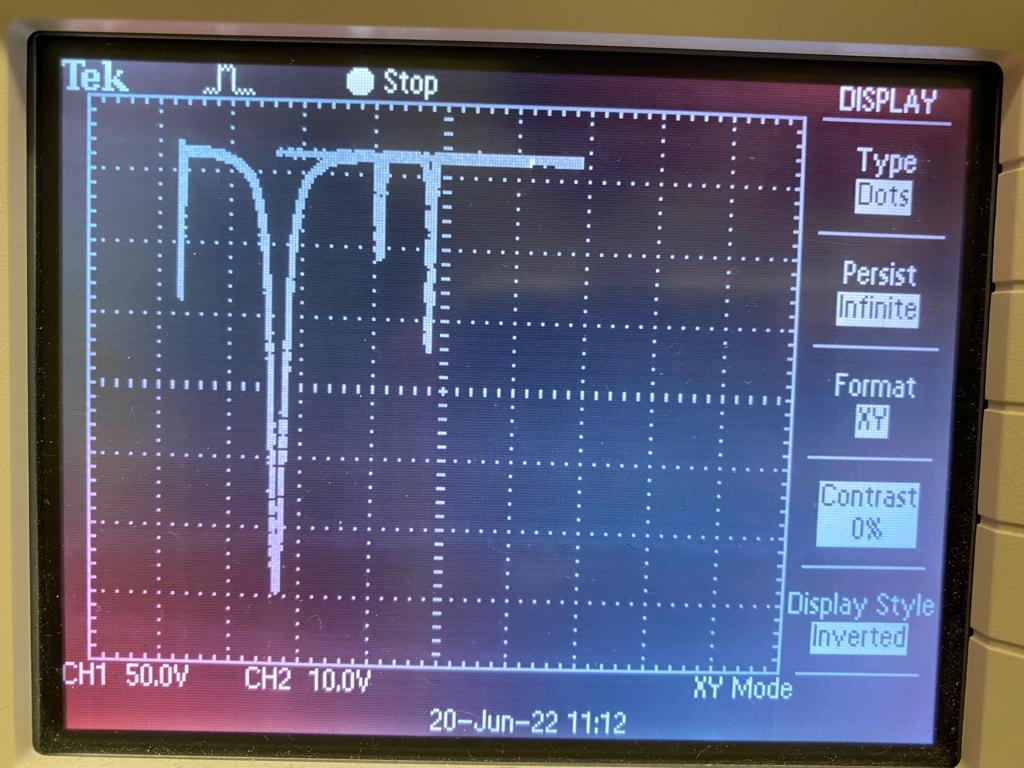
\includegraphics[width = 0.7 \textwidth]{data_scripts/index.jpg}
\end{figure}
In Abbildung \ref{fig:transmissionsspektrum} können die Tiefen der Peaks im Vergleich zum Nullniveau abgelesen werden.
Für das Isotop $^{85}\text{Rb}$ kann die Anzahl der Striche zu $N_{85}=13$ gezählt werden, während 
$N_{87} = 7$ Striche für das Isotop $^{87}\text{Rb}$ gezählt werden.
Somit beträgt das Verhältnis ca. $\qty{50}{\percent}$, womit gesagt werden kann, dass 
das $^{85}\text{Rb}$ ca. $\frac{2}{3}$ und $^{87}\text{Rb}$ ca. $\frac{1}{3}$ ausmacht.
\subsection{Quadratischer Zeemann-Effekt}
Die Aufspaltung durch den quadratischen Zeemann-Effekt kann bei den maximalen Feldstärken 
$B_{\text{max},85} = \qty{239.48}{\micro\tesla}$ und $B_{\text{max},87} = \qty{162.32}{\micro\tesla}$ mittels \eqref{eqn:zeem} bestimmt werden.
Dabei gilt $M_{F, 85} = 3$ und $M_{F, 87} = 2$.
Die Energiedifferenzen beim quadratischen Zeemann-Effekt können somit als
\begin{align*}
    \symup{\Delta}E_{\text{Z}, 85} &= \qty{4.57(1386)}{\nano\electronvolt} \\
    \symup{\Delta}E_{\text{Z}, 87} &= \qty{4.70(940)}{\nano\electronvolt} 
\end{align*} 
angegeben werden.
